\chapter{Metodologia}
\label{cap:metodologia}

\section{Escopo do Experimento}
\label{sec:escopo}

O escopo deste experimento é definido a partir do paradigma \textit{Goal Question Metric} (GQM) \cite{basili1994gqm}. O objetivo é formulado como: analisar \textit{guardrails} baseados em LLM, com o propósito de avaliá-los, com relação à eficácia na classificação de conteúdo prejudicial, do ponto de vista de pesquisadores e desenvolvedores, no contexto de modelos submetidos a diferentes níveis de quantização via AWQ, operando sobre entradas em inglês e em português brasileiro.

\section{Design Experimental}
\label{sec:design}

Este trabalho adota o framework de experimentos controlados em Engenharia de Software proposto por \citeonline{wohlin2012experimentation}, adaptado para o contexto de experimentos computacionais com modelos de linguagem. Nessa adaptação, os modelos de linguagem assumem o papel de sujeitos empíricos, pois são eles que executam a tarefa de classificação sobre os objetos do experimento. Essa escolha é declarada explicitamente pois o framework original foi concebido para experimentos com participantes humanos, e sua adaptação para agentes computacionais implica diferenças metodológicas discutidas ao longo desta seção.

O experimento segue um design fatorial completo, em que todas as combinações possíveis entre os fatores são avaliadas, totalizando 30 configurações experimentais, conforme ilustrado na Figura~\ref{fig:design-fatorial}. A ordem de inferência não foi aleatorizada, pois, sob as restrições do protocolo definido na Seção~\ref{sec:protocolo}, cada prompt é processado de forma independente, eliminando efeitos de aprendizado ou fadiga que justificariam a aleatorização em experimentos com sujeitos humanos.

\begin{figure}[h!]
	\Caption{\label{fig:design-fatorial} Design fatorial do experimento}
	\UFCfig{}{
		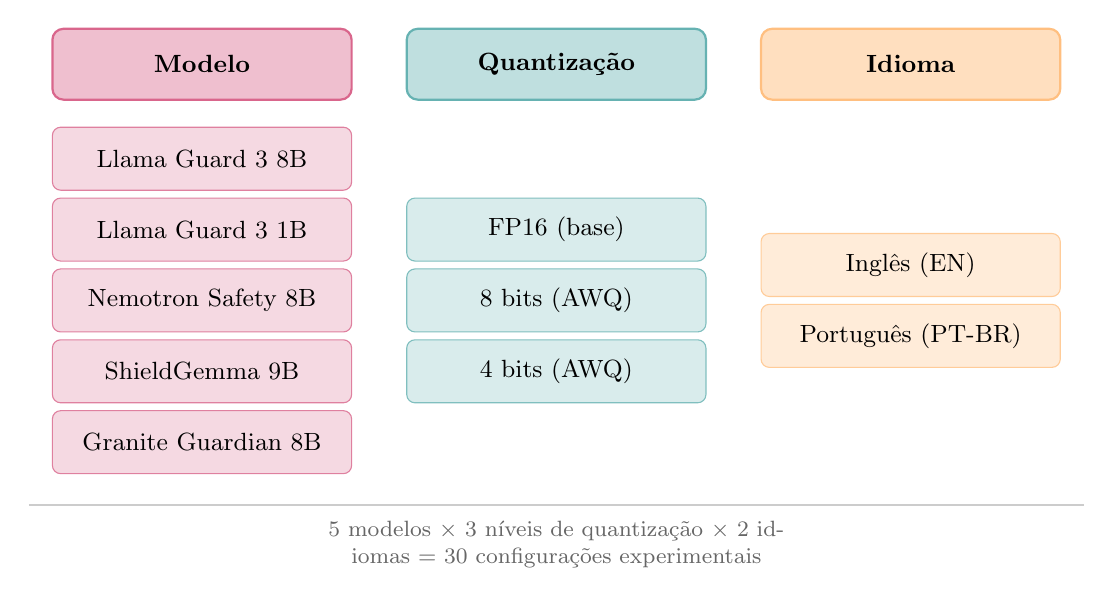
\begin{tikzpicture}[
			font=\small,
			factor/.style={rectangle, rounded corners=4pt, minimum width=3.8cm, minimum height=0.9cm, text centered, draw=black!60, thick},
			level/.style={rectangle, rounded corners=3pt, minimum width=3.8cm, minimum height=0.8cm, text centered, draw=black!40},
			modelo/.style={level, fill=purple!15, draw=purple!50},
			quant/.style={level, fill=teal!15, draw=teal!50},
			idioma/.style={level, fill=orange!15, draw=orange!40},
			fator_modelo/.style={factor, fill=purple!25, draw=purple!60},
			fator_quant/.style={factor, fill=teal!25, draw=teal!60},
			fator_idioma/.style={factor, fill=orange!25, draw=orange!50},
			]
			\node[fator_modelo] (fm) at (0,0)     {\textbf{Modelo}};
			\node[fator_quant]  (fq) at (4.5,0)   {\textbf{Quantização}};
			\node[fator_idioma] (fi) at (9,0)      {\textbf{Idioma}};
			\node[modelo] (m1) at (0,-1.2)  {Llama Guard 3 8B};
			\node[modelo] (m2) at (0,-2.1)  {Llama Guard 3 1B};
			\node[modelo] (m3) at (0,-3.0)  {Nemotron Safety 8B};
			\node[modelo] (m4) at (0,-3.9)  {ShieldGemma 9B};
			\node[modelo] (m5) at (0,-4.8)  {Granite Guardian 8B};
			\node[quant] (q1) at (4.5,-2.1) {FP16 (base)};
			\node[quant] (q2) at (4.5,-3.0) {8 bits (AWQ)};
			\node[quant] (q3) at (4.5,-3.9) {4 bits (AWQ)};
			\node[idioma] (i1) at (9,-2.55) {Inglês (EN)};
			\node[idioma] (i2) at (9,-3.45) {Português (PT-BR)};
			\draw[black!20, thick] (-2.2,-5.6) -- (11.2,-5.6);
			\node[text width=10cm, text centered, font=\footnotesize, text=black!60] 
			at (4.5,-6.1) 
			{5 modelos $\times$ 3 níveis de quantização $\times$ 2 idiomas = 30 configurações experimentais};
		\end{tikzpicture}
	}{
		\Fonte{Elaborado pelo autor.}
	}
\end{figure}

\subsection{Fatores e Tratamentos}
\label{sec:fatores}

Os fatores deste experimento são as variáveis independentes efetivamente manipuladas. Vale observar que o fator modelo assume um duplo papel neste design: os modelos são simultaneamente sujeitos, pois executam a tarefa de classificação, e um fator experimental, pois seu tipo é uma variável independente do experimento. Essa sobreposição é característica de estudos comparativos entre sistemas computacionais e não compromete o design fatorial adotado.

O primeiro fator é o \textbf{modelo}, cujos cinco níveis correspondem aos cinco \textit{guardrails} selecionados e detalhados na Seção~\ref{sec:modelos}. O segundo fator é o \textbf{nível de quantização}, com três níveis: precisão base em 16 bits (FP16), quantização em 8 bits e quantização em 4 bits, todos aplicados via AWQ. O terceiro fator é o \textbf{idioma}, com dois níveis: inglês (EN) e português brasileiro (PT-BR).

Algumas variáveis independentes foram mantidas fixas ao longo de todo o experimento, 
não constituindo fatores, mas sendo registradas como variáveis de controle para 
garantir a reprodutibilidade dos resultados. São elas: temperatura de inferência 
fixada em zero, garantindo comportamento determinístico dos modelos; conjunto de 
calibração AWQ padronizado (Pile); e modo de classificação de entrada 
(\textit{input classification}), aplicado uniformemente a todos os modelos.

\subsection{Variáveis Dependentes}
\label{sec:variaveis}
As variáveis dependentes são as métricas que capturam o efeito dos tratamentos sobre o desempenho dos modelos na tarefa de classificação de conteúdo prejudicial. As métricas primárias são precisão (\textit{precision}), revocação (\textit{recall}) e F1-score, calculadas para cada uma das 30 configurações experimentais. A métrica derivada central é o $\Delta\text{F1}$, definido como a diferença entre o F1 obtido em inglês e o F1 obtido em português brasileiro para uma mesma configuração de modelo e nível de quantização, e que operacionaliza diretamente a pergunta de pesquisa deste trabalho. As fórmulas e procedimentos de cálculo dessas métricas são detalhados na Seção~\ref{sec:metricas}.


\section{Hipóteses}
\label{sec:hipoteses}
\textcolor{red}{TODO: formalizar H0 e H1 para cada hipótese — definir testes estatísticos antes de escrever}

\section{Dataset}
\label{sec:dataset}
% BeaverTails, tradução GPT-4o, fallback no\_translate, 
% distribuição de classes (~44\% safe / 55\% unsafe), 14 categorias

\section{Modelos}
\label{sec:modelos}
% Os 5 modelos, justificativa de seleção, classificação multilíngue

\section{Quantização}
\label{sec:quantizacao}
% AWQ via vLLM, níveis 16bit/8bit/4bit, calibração Pile padrão
% Justificar exclusão do 2bit

\section{Protocolo de Inferência}
\label{sec:protocolo}
% Temperatura 0, modo input classification, formato de prompt

\subsection{Ambiente de Execução}
\label{sec:ambiente}
\textcolor{red}{TODO: especificar GPU (L40S), VRAM, SO, versões de PyTorch, vLLM e AWQ}

\subsection{Experimento Piloto}
\label{sec:piloto}
\textcolor{red}{TODO: descrever execução em menor escala para validar pipeline vLLM, 
	parsing das respostas e estimativa de tempo total}

\section{Métricas e Procedimentos de Análise}
\label{sec:metricas}
% F1, precision, recall, Delta F1
\textcolor{red}{TODO: definir testes estatísticos para validação das hipóteses 
	— resolver questão do experimento determinístico sem repetições}

\section{Ameaças à Validade}
\label{sec:ameacas}
\textcolor{red}{TODO: mapear validade interna, externa e de construto}